
\chapter{Fundamentos Teóricos}

En esta sección vamos a introducir cuales serían los conceptos teóricos más importantes que conviene tener presentes para la correcta comprensión del trabajo y sus resultados. Para ello se ha recurrido al conocimiento adquirido en asignaturas como \textbf{Visión por Computador}, \textbf{Aprendizaje Automático} así como diversos artículos que se citarán dónde sea conveniente.

\section{Aprendizaje Automático}
    \noindent Actualmente la \textbf{Inteligencia Artificial} (IA) es una rama de la informática muy popular y de gran importancia que pretende dotar a los ordenadores de una manera de razonar o solucionar problemas inteligente. En este contexto, la IA ha explorado diversos métodos para conseguir este propósito como son el estudio de Metaheurísticas, la Ingeniería del Conocimiento y más recientemente el conocido \textbf{Aprendizaje Automático} (AA). 
    
    \medskip

    \noindent Los métodos que empleamos en este trabajo pretenecen a la rama del AA, y por lo tanto es importante comenzar definiendo qué es este concepto. Para ello, disponemos de diversas definiciones proporcionadas por distintos autores: 

    \medskip

    \noindent La primera y más clásica nos la proporciona Arthur Samuel en 1959, en la cual define el AA como \textbf{el campo de estudio que da a los ordenadores la capacidad de aprender sin ser programados explícitamente}. Esta definición es muy general, pero nos permite hacernos una idea de lo que pretende conseguir este campo de estudio, que es dotar a los ordenadores de la capacidad de \entrecomillado{aprender}, generalmente a partir de una base de datos, con la idea de poder usar este conocimiento adquirido durante el aprendizaje para resolver casos nuevos del problema que la máquina no conozca previamente.
    
    \medskip

    \noindent Una definición un poco más reciente de Tom Mitchell (1998) nos dice que: \textbf{Un programa de ordenador se dice que aprende de la experiencia E respecto de alguna tarea T y alguna medida de rendimiento P, si su rendimiento en T, medido por P, mejora con la experiencia E}. Esta segunda definición nos permite identificar los elementos necesarios para poder resolver un problema mediante técnicas de AA. Así, en primer lugar necesitamos una tarea (T) que queremos resolver con ayuda de un ordenador, una experiencia (E) en esa tarea, que generalmente es una base de datos asociada al problema, y una medida de rendimiento (P) que generalmente se asocia con una función objetivo que se pretende minimizar/maximizar.

    \medskip

    \noindent Tradicionalmente, los algoritmos de AA se dividen en dos conjuntos:

    \begin{itemize}
        \item Aprendizaje Supervisado.
        \item Aprendizaje no Supervisado.
    \end{itemize}

    \medskip 
    
    \noindent No obstante, han aparecido otras técnicas más recientes como el Aprendizaje por Refuezo que son muy interesantes y usadas actualmente, pero no vamos a profindizar en ellas pues no son necesarias para el trabajo que nos ocupa.

    \subsection{Aprendizaje Supervisado}
        \noindent Los algoritmos de AA que se emplean en este conjunto se caracterizan porque disponen de una base de datos \textbf{etiquetados} de manera que para cada dato $x$ conocemos su etiqueta asociada $y$, y nuestro objetivo sería tratar de conocer la función $f$ que los relaciona, de manera que $f(x)=y$.

        \medskip

        \noindent Dentro de este grupo podemos encontrar problemas de \textbf{regresión} y de \textbf{clasificación}.

        \subsubsection{Regresión} \label{section::Regresion}
            \noindent En los problemas de regresión se pretende obtener la función $f$ que asocia correctamente a cada dato su etiqueta: 
            \begin{equation}
                f(x)=y \; \; con \; \; x\in \mathbb{R}^m \; \; y \in \mathbb{R}^n
            \end{equation}
            
            \noindent Generalmente, obtener la función $f$ exacta es complicado, por lo que se pretende aproximar mediante una función $f'$ que elegimos y que entrenaremos a partir de los datos etiquetados que se nos proporcionan. Volviendo a la definición de Tom Mitchell, en este tipo de problemas tendríamos que 
            
            \begin{itemize}
                \item T= regresión (aproximar $f$)
                \item E= El conjunto de datos $X$ etiquetados que se proporcionan para entrenar el modelo $f'$.
                \item P= función de coste asociada (generalmente se emplea el error cuadrático medio) que nos mide lo \entrecomillado{bien} que nuestra función $f'$ aproxima a $f$.
            \end{itemize}
            
            \medskip 

            \noindent Por ejemplo el si intentamos predecir $f$ mediante un modelo lineal: 

            \begin{equation}
                f'(x)= w^T x \; \; x,w \in \mathbb{R}^m
            \end{equation}

            \noindent Disponemos de un conjunto de $N$ datos 
            
            \begin{equation}
                X= \lbrace x_1, x_2 , \ldots , x_N \rbrace \; \; x_i \in \mathbb{R}^m
            \end{equation}

            \noindent Además de un conjunto de etiquetas

            \begin{equation}
                Y= \lbrace y_1, y_2 , \ldots , y_N \rbrace \; \; y_i \in \mathbb{R}^n
            \end{equation}

            \noindent Y usamos como medida de error el error cuadrático medio: 

            \begin{equation}
               J(\alpha)= \frac{1}{N} \sum_{i=1}^{N}(f'(x_i) - f(x_i))^2 = \frac{1}{N} \sum_{i=1}^{N}(y_i' - y_i)^2
            \end{equation}

            \noindent Dónde $y_i'$ es la etiqueta predicha por $f'$ para $x_i$.

            \medskip

            \noindent Nuestro objetivo sería encontrar el vector de pesos $w$ que minimice la función de coste $J$ y para ello utilizamos los datos de entrenamiento $X$.
            
        \subsubsection{clasificación}
            \noindent Por otro lado tenemos los problemas de clasificación, en los datos se encuentran agrupados en clases y se pretende clasificar cada dato de entrada en la clase correcta. Los casos más sencillos de este problema son los de \textbf{clasificación binaria}, y en ellos se pretende agrupar los datos en dos posibles clases que suelen codificarse como $0$ y $1$.

    \subsection{Aprendizaje no Supervisado}
            \noindent El aprendizaje no supervisado se caracteriza porque los datos que se proporcionan no están etiquetados, y no se busca una salida concreta, sino que se pretende analizar las características de nuestro conjunto de datos. 

            Así, por ejemplo, tareas que pueden resolverse con esta técnica pueden ser la agrupación de clientes de cierta compañía en distintas clases según sus características.
            
    \subsection{Nuestro Problema}
        \noindent En nuestro problema, los frameworks de los que disponemos resuelven problemas de aprendizaje supervisado y no supervisado. 
        
        \medskip
        
        \noindent Por ejemplo vamos a intentar predecir los landmarks cefalométricos para una cierta imagen de entrada, lo que nos llevaría a un problema típico de aprendizaje supervisado en el que pretendemos a partir de la imagen de entrada conocer la función que nos proporciona la salida correcta (la imagen con los landmarks marcados correctametne).

        \medskip

        \noindent Por otro lado, uno de nuestros frameworks tiene una etapa de entrenamiento previa al problema de los landmarks en la cual mediante conjuntos de datos de imágenes sin etiquetar de rostros humanos, se pretende reconstruir imágenes preservando al máximo posible la estructura de la cara. Esto, como podemos ver, es un problema típico de aprendizaje no supervisado, porque no se busca obtener una etiqueta para cada imagen, sino analizar la estructura de los distintos elementos de los datos de entrada para ser capaces de reconstruirlos preservando su estructura.

    \subsection{Gradiente Descendente}
        \noindent En esta sección hemos hablado de qué es el AA y cómo se formalizan sus problemas para poder resolverlos. Y en concreto hemos formalizado cómo se resuelven los problemas de regresión en los que queríamos aproximar una función desconocida $f$ a partir de una aproximación $f'$ y en base a una función de coste. Sin embargo, no hemos hablado de ningún algoritmo que se use en la minimización de dicha función de coste. Es por ello que vamos a explicar el principal algoritmo que se utiliza para esta tarea, el \textbf{Gradiente Descendente}. 

        \medskip

        \noindent El Gradiente descendente es un algoritmo clásico que persigue la idea intuitiva de que el gradiente de una función siempre \entrecomillado{apunta} hacia el máximo de esta, por lo que seguir la dirección contraria a este nos llevará al mínimo de la función. Más formalmente, si recuperamos la notación del apartado \autoref{section::Regresion} tendríamos: 

        \medskip
        
        \noindent La función objetivo es: 
        \begin{equation}
            f(x)=y \; \; x \in \mathbb{R}^m \; \; y \in \mathbb{R}^n
        \end{equation}

        \noindent La función con la que vamos a intentar aproximar la función objetivo es:
        \begin{equation}
            f'(x,w)=y \; \; x \in \mathbb{R}^m \; \; y \in \mathbb{R}^n \; \; w \in \mathbb{R}^d 
        \end{equation}

        \noindent La función de coste sería $J(w)$ que de alguna manera mide la distancia entre $f$ y $f'$ y que para poder aplicar el método debe ser derivable. Algunas funciones de coste usuales son: 

        \begin{itemize}
            \item La función \textbf{L2} (también conocida como error cuadrático medio): 
            \begin{equation}
                J(w)=\frac{1}{N} \sum_{i=1}^N(f(x_i,w)-f'(x_i))^2
            \end{equation}
            \item La función \textbf{L1} (también conocida como error absoluto medio): 
            \begin{equation}
                J(w)=\frac{1}{N} \sum_{i=1}^N \left|f(x_i,w)-f'(x_i)\right|
            \end{equation}
        \end{itemize}

        \noindent Una vez hemos formalizado el problema, el algoritmo \textbf{Gradiente Descendente} consiste en: 

        \begin{itemize}
            \item Se inicializa el vector de pesos $w$.
            \item En cada paso $i$ del entrenamiento, el vector de pesos del siguiente paso $i+1$ se calcula de acuerdo a la siguiente relación: 
            \begin{equation}
                w_{i+1}=w_i-\eta \nabla J(w)
            \end{equation}
            \noindent Dónde $\eta$ es un factor conocido como \textbf{learning rate}(lr) que mide el \entrecomillado{tamaño} del paso que en cada iteración damos en búsqueda del mínimo. 
        \end{itemize}

        \noindent Idealmente, con este método se encuentra un mínimo global de la función de coste en el caso en que esta sea convexa. En caso de no serlo podría caer en un mínimo local en su lugar. 

        \medskip

        \noindent Por otro lado, cabe destacar la importancia de una buena elección del \textbf{learning rate}, pues si este es demasiado pequeño puede ocasionar una lenta convergencia al mínimo, y por lo tanto que se realice un gran número de iteraciones, y en cambio un valor excesivamente grande de este puede impedir la convergencia,pues los saltos serían tan grandes en la dirección del mínimo local o global que podría llegar a \entrecomillado{saltar} por encima de este siempre. Por lo tanto una técnica habitual aunque costosa de este algoritmo consiste en usar un learning rate adaptativo, que sea mayor en las primeras iteraciones y que vaya disminuyendo conforme se incremente el número de iteraciones (pues se entiende que se estará cerca del mínimo).

        \subsubsection{Gradiente Descendente Estocástico}

            \noindent El algoritmo descrito anteriormente tiene el problema de ser costoso computacionalmete, debido a que en cada iteración se debe calcular la función de coste para todos los ejemplos del conjunto de entrenamiento $X$. Es por ello que suele emplearse en su lugar una versión modificada y que sigue dando buenos resultados que consiste en actualizar los pesos en base a unos pocos ejemplos del conjunto de entrenamiento $X$ que se conoce como \entrecomillado{minibatch}.




\section{Visión por Computador}
    \noindent La \textbf{Visión por computador} es un área de conocimiento en el que se unen diversas disciplinas como la IA o el AA para un propósito común, que es el procesado de imágenes por medio de un ordenador con la finalidad de que la máquina pueda llegar a extraer información relativa a estas del mismo modo en que lo haría un ser humano \cite{rosenfeld1988computer}. 

    \medskip
    
    \noindent Problemas clásicos de la visión por computador son el reconocimiento de objetos o personas en imágenes, la segmentación o la clasificación. Así pues, podemos ver la relación directa que hay entre nuestro objetivo y esta disciplina, pues los frameworks que usaremos tendrán por objetivo extraer información de imágenes de rostros de personas para posteriormente tratar de identificar en ellos con el mayor grado de decisión posible una serie de landmarks cefalométricos que el sistema ha aprendido a base de unos ejemplos etiquetados (AA).

    \medskip

    \noindent Finalmente, en los últimos años esta rama ha experimentado un fuerte crecimiento e importancia en la comunidad científica debido al actual desarrollo del \textbf{Deep Learning} y las \textbf{redes convolucionales profundas} que explicaremos en detalle en la siguiente sección. Estas nuevas herramientas han permitido crear programas que obtienen un gran rendimiento en el tratamiento de imágenes. Ejemplo de ello son los dos frameworks que vamos a comparar en este trabajo.

\section{Deep Learning}
    Como ya se ha mencionado anteriormente, la IA se encuentra muy desarrollada actualmente y es capaz de resolver problemas que tradicionalmente eran muy complicados para ser resueltos por un humano, pero que se ha demostrado que no son tan complicados para una máquina. Sin embargo, e irónicamente, algunas de las tareas más fáciles para los seres humanos como son el reconocimiento del habla o la identificación de objetos en imágenes han suponen un verdadero reto para un odernador, y o ha sido hasta los últimos años con el nacimiento del \textbf{Deep Learning} que se han empezado a obtener resultados satisfactorios en este campo.
    
    Por lo tanto, los algoritmos del Deep Learning se caracterizan por resolver estos problemas a partir de representaciones del mismo que se expresan en terminos de otras más simples. De esta manera se pueden construir conceptos difíciles a partir de otros más sencillos. Este grafo puede ser tan profundo como se necesite, por ello se le conoce como Deep Learning.

    \subsection{Redes Neuronales}
        La arquitectura básica de los modelos de Deep Learning viene descrita por la arquitectura de una \textbf{red neuronal}. Es por ello que vamos a profundizar un poco en esta estructura y para ello vamos a partir de un ejemplo clásico como es el \textbf{Perceptrón multicapa}(MLP). Para esta sección vamos a seguir el capítulo 6 de \cite{Goodfellow-et-al-2016}.

        \medskip

        \noindent Las redes neuronales tienen por objetivo aproximar una función desconocida $f(x)=y$ que asocia a cada entrada $x$ una salida $y$ a partir de una función $f'(x;W)= \widehat{y}$ (dónde $\widehat{y}$ es la etiqueta predicha para la entrada $x$) que depende de unos parámetros $W$, de manera que el objetivo es aprender los valores de $W$ que mejor aproximan la función objetivo $f$.

        \medskip

        \noindent Se denominan algoritmos \textbf{feedforward} porque la información fluye desde la entrada $x$ a través de los cálculos intermedios que definen $f'$ hasta finalmente dar una salida $y$.

        \medskip

        \noindent Finalmente a estos algoritmos se les denomina \textbf{redes} porque generalmente se representan como una composición de distintas funciones en cadena de manera que se van aplicando sucesivamente sobre la entrada $x$ hasta la salida $\widehat{y}$. 

        \begin{figure}[!h]
            \centering
            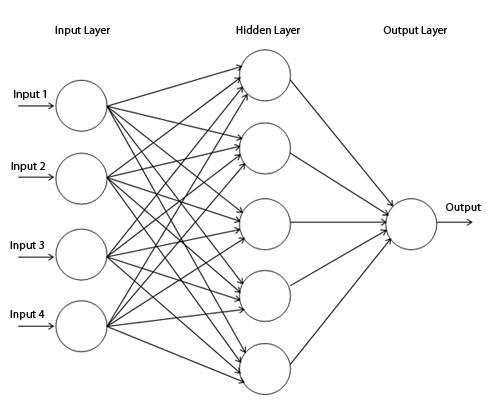
\includegraphics[width=0.5\textwidth]{img/single_hidden_layer.jpg}
            \caption{Red neuronal con una capa oculta. Formalmente podría describirse como $f'(x)=(f_3(f_2(f_1(x))))$, dónde $f_1$ hace referencia a la capa de entrada a la red, $f_2$ a la capa oculta y $f_3$ a la capa de salida.}
            \label{fig:red_neuronal_capa_oculta}
          \end{figure}

        \noindent La \textbf{profundidad} de la red vendría dada por la cantidad de \textbf{capas ocultas} que esta tiene. En los algoritmos de Deep Learning veremos un gran número de capas ocultas, de ahí el nombre. 

        \medskip

        \noindent Por otro lado, cada capa contiene un número determinado de \textbf{neuronas}, que se relacionan con las de la capa siguiente y las de la capa anterior mediante combinaciones lineales generalmente. Sin embargo, estas combinaciones lineales no son suficientes para que la red pueda aproximar funciones objetivo $f$ que sean no-lineales, para ello se emplean las llamadas \textbf{funciones de activación}. Se tratan de un conjunto de funciones no-lineales entre las que destacan las siguientes \cite{sharma2017activation}: 

        \begin{itemize}
            \item \textbf{Función Sigmoide}. Transforma los valores de entrada a un valor entre $0$ y $1$.
            \begin{equation}
                Sigmoide(x)=\frac{1}{e^{-x}}
            \end{equation}
            \item \textbf{Función Tangente Hiperbólica}. Es similar a la función sigmoide, pero es simétrica respecto al origen. 
            \begin{equation}
                tanh(x)=\frac{e^x - e^{-x}}{e^x + e^{-x}} 
            \end{equation}
            \item \textbf{Función ReLU}. Es una de las más usadas en redes neuronales por ser de las más eficientes, ya que permite que no se activen todas las neuronas a la vez, ya que en aquellas cuya salida tras la combinación lineal con los pesos de la capa correspondiente sea 0 no serán activadas.
            \begin{equation}
                ReLU(x)=\max(0,x)
            \end{equation}

            \noindent Existe el problema de que en algunos casos, el gradiente de la función sea $0$ debido a que los pesos no se actualicen durante el proceso que explicaremos más adelante de \textbf{back-propagation}.

            \item \textbf{Función Leaky ReLU}. Es una versión mejorada de la función anterior, ya que para los casos en los que la función anterior valía $0$, ahora se expresan como una componente lineal de la entrada $x$ muy pequeña, de esta manera se resuelve el problema de que el gradiente de la función sea $0$. 
            \begin{equation}
                LeakyReLU(x)=\left\{ \begin{array}{lcc}
                    x &   si  & x \leq 0 \\
                    \\ ax &  si & 0 < x \\
                    \end{array}
                \right.
            \end{equation}

            \noindent Dónde $a$ es un valor muy próximo a $0$.
            \item \textbf{Función SoftMax}. Es una combinación de múltiples funciones sigmoide. Mientras que la función Sigmoide se usa en problemas de clasificación binaria, la función SoftMax permite que se pueda realizar clasificación multiclase, ya que transforma un vector de entrada K-dimensional de valores reales en un vector K-dimensional de elementos entre $0$ y $1$, de manera que la componente más próxima a $1$ podría entenderse como la clase a la que pertenecería el elemento en un problema de clasificación multiclase.
            
            \begin{equation}
                \sigma(x)_j= \frac{e^{z_j}}{\sum_{k=1}^{K}e^{z_k}} \; \; j=1, \ldots, K
            \end{equation}
        \end{itemize}

        \noindent No existe una manera de elegir la mejor función para cada caso, pero de forma experimental se ha podido comprobar que la función ReLU en general da buenos resultados y si hubiera demasiadas neuronas muertas en la red podría cambiarse por la Leaky ReLU.

        \medskip

        \noindent De esta manera, en la capa $i$ de la red, la función $f_i$ suele tener la siguiente expresión: 

        \begin{equation}
            f_i(x)=\gamma(w_i^T x)
        \end{equation}

        \noindent Dónde $\gamma$ representa una función cualquiera del conjunto de funciones de activación que hemos descrito antes y $w_i$ el vector de pesos correspondiente a la capa $i$ de la red.
    
    \subsection{Back Propagation}
        Todas las funciones de las capas intermedias de la red son derivables, por lo que se podría calcular de forma explícita su expresión en cada caso, lo que ocurre es que este proceso es costoso computacionalmete. En lugar de esto se aplica la técnica de \textbf{Back-propagation}.

        \medskip

        \noindent Para entender este proceso correctamente se debe introducir primero el concepto de \textbf{Grafo Computacional}, que no es otra cosa que representar una función mediante un grafo. Como por ejemplo \autoref{fig:GrafoComputacional}.

        \begin{figure}[!h]
            \centering
            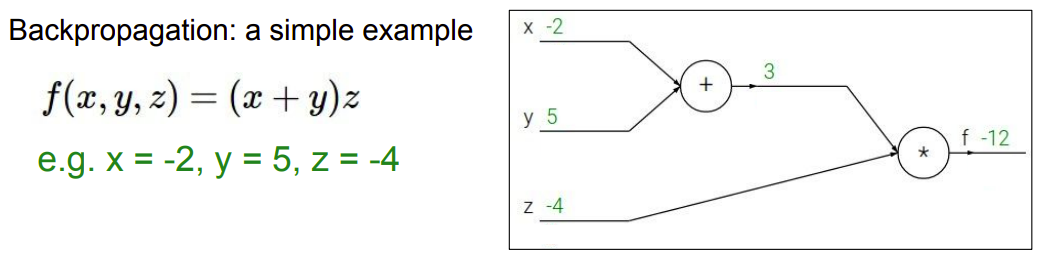
\includegraphics[width=0.8\textwidth]{img/GrafoComputacional.png}
            \caption{Ejemplo de Grafo computacional junto con la salida para una entrada concreta $x=-2$,$y=5$, $z=-4$. La imagen ha sido extraida del curso \cite{StanfordCourse}.}
            \label{fig:GrafoComputacional}
        \end{figure}

        \medskip

        \noindent La idea del algoritmo de Back-propagation es ir calculando la derivada en cada nodo del grafo computacional mediante la aplicación de la regla de la cadena, de manera que si $f(x,y,z)=g(x,y)h(z)$ si quisiéramos calcular $\frac{\partial f}{\partial x}$ aplicando la regla de la cadena tendríamos que: 

        \begin{equation}
            \frac{\partial f}{\partial x}= \frac{\partial f}{\partial g} \frac{\partial g}{\partial x}
        \end{equation}

        
        Podemos entender mejor el proceso resolviendo el ejemplo \autoref{fig:GrafoComputacional}: 

        \begin{figure}[!h]
            \centering
            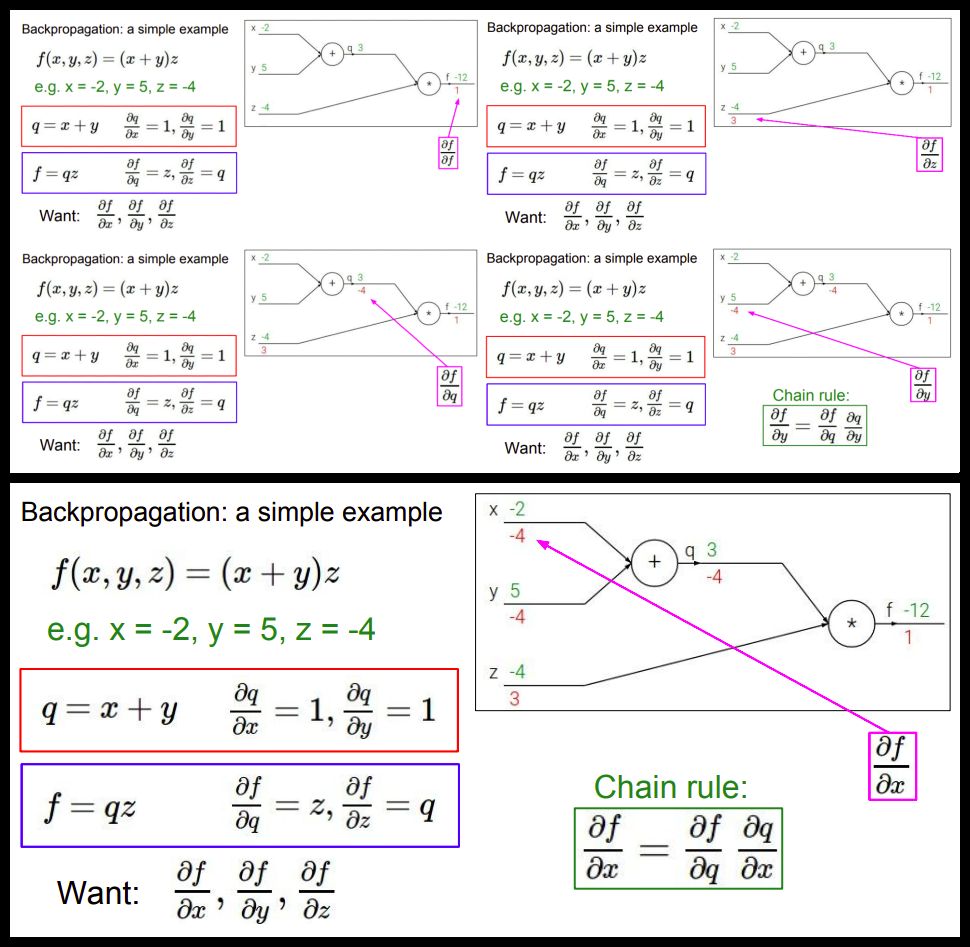
\includegraphics[width=0.8\textwidth]{img/BP_ejemplo.png}
            \caption{Como podemos ver en la imagen superior, en primer lugar se renombra la salida de la operación $x+y$ por $q$, de manera que $f=qz$. Tras esto se empiezan a calcular las derivadas parciales correspondientes desde el final hacia la entrada, aplicando cuando sea necesario la regla de la cadena hasta obtener la derivada de cada nodo en la imagen de abajo. Las imágenes han sido extraidas de \cite{StanfordCourse}}
            \label{fig:Ejemplo BP}
        \end{figure}

        \noindent Como vemos en \autoref{fig:Ejemplo BP}, se produce un flujo desde la salida hacia la entrada en la que se van calculando los gradientes para cada parámetro. Una vez calculado el gradiente se procede a actualizar los pesos usando por ejemplo el algoritmo de \textbf{gradiente descendente}.
    
\section{Redes Neuronales Convolucionales Profundas}
    \subsection{Capa Convolucional}

    \subsection{Capa de Pooling}

    \subsection{Capa Totalmente Conectada}

    \subsection{Evolución Histórica de las CNN}

    \subsection{Optimizadores empleados}

\section{Adversarial Autoencoder}
    \subsection{Evolución Histórica}

\section{Tratamiento de imágenes 2D y técnicas empleadas}
    \subsection{Tratamiento de imágenes 2D}

    \subsection{Data Augmentation}

    \subsection{few-shot Learning}

\endinput
%------------------------------------------------------------------------------------
% FIN DEL CAPÍTULO. 
%------------------------------------------------------------------------------------

